\subsection{Упражнение 1}

Запустите и прослушайте примеры в файле chap03.ipynb. В примере с утечкой попробуйте заменить окно Хэмминга одним из других окон, предоставляемых NumPy, и посмотрите, как они влияют на утечку.

\begin{lstlisting}[language=Python]
signal = SinSignal(freq=440)
duration = signal.period * 30.25
wave = signal.make_wave(duration)
spectrum = wave.make_spectrum()
spectrum.plot(high=880)
\end{lstlisting}

\begin{figure}[H]
	\begin{center}
		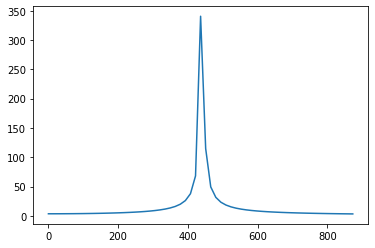
\includegraphics[scale=1]{fig/lab03/lab03_1.png}
		\caption{Рассматриваемый сигнал}
	\end{center}
\end{figure}

Посмотрим как выглядит спектограмма с использованием окна Хэмминга:

\begin{figure}[H]
	\begin{center}
		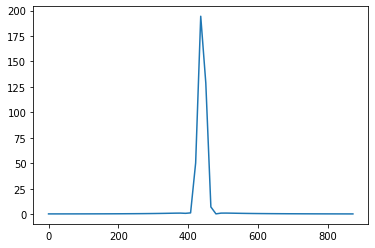
\includegraphics[scale=1]{fig/lab03/lab03_2.png}
		\caption{Сигнал с использованием окна Хэмминга}
	\end{center}
\end{figure}


Используем другое окно а именно Барлетта

\begin{lstlisting}[language=Python]
wave = signal.make_wave(duration)
wave.ys *= np.bartlett(len(wave.ys))
spectrum = wave.make_spectrum()
spectrum.plot(high=880)
\end{lstlisting}
\begin{figure}[H]
	\begin{center}
		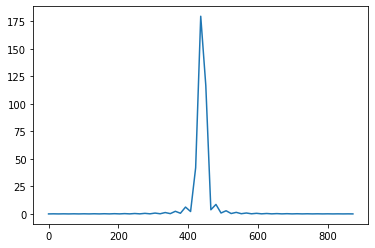
\includegraphics[scale=1]{fig/lab03/lab03_3.png}
		\caption{Сигнал с использованием окна Барлетта}
	\end{center}
\end{figure}

Можно заметить. что низкие амплитуды стали ломанными линиями.

\subsection{Упражнение 2}


Напишите класс SawtoothChirp, расширяющий Chirp и переопределяющий evaluate для генерации пилообразного сигнала с линейно увеличивающейся частотой.

\begin{lstlisting}[language=Python]
import thinkdsp
from thinkdsp import normalize, unbias
from math import pi

class SawtoothChirp(Chirp):

    def evaluate(self, ts):
        freqs = np.linspace(self.start, self.end, len(ts))
        dts = np.diff(ts, prepend=0)
        dphis = (2 * np.pi) * freqs * dts
        phases = np.cumsum(dphis)
        cycles = phases / (2 * np.pi)
        frac, _ = np.modf(cycles)
        ys =  normalize(unbias(frac), self.amp)
        return ys
\end{lstlisting}

Создадим пилообразный сигнал от второй до пятой октавы "ля" 880 - 7040.

\begin{lstlisting}[language=Python]
signal = SawtoothChirp(start=880, end=7040)
wave = signal.make_wave(duration=3, framerate=4000)
wave.apodize()
wave.make_audio()
sp = wave.make_spectrogram(seg_length=512)
sp.plot(high=5000)
\end{lstlisting}

\begin{figure}[H]
	\begin{center}
		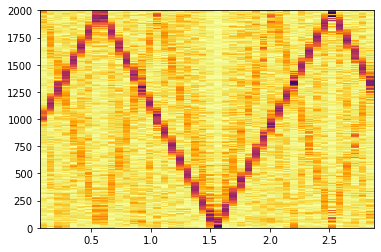
\includegraphics[scale=1]{fig/lab03/lab03_4.png}
		\caption{Спектр сигнала}
	\end{center}
\end{figure}

По звуку и эскизу виден эффект биения.


\subsection{Упражнение 3}

Создайте пилообразный чирп, меняющийся от 2500 до 3000 Гц, и на его основе сгенерируйте сигнал длительностью 1 с и частотой кадоров 20 кГц. Нарисуйте, каким примерно будет Spectrum. Затем распечатайте Spectrum и посмотрите, правы ли вы.

\begin{lstlisting}[language=Python]
sawC = SawtoothChirp(start=2500, end=3000)
wave = sawC.make_wave(duration=1, framerate=20000)
wave.make_spectrum().plot()
\end{lstlisting}
\begin{figure}[H]
	\begin{center}
		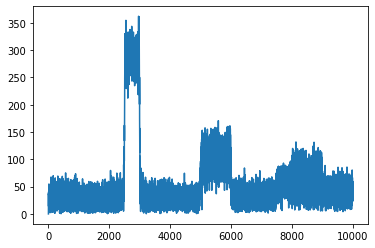
\includegraphics[scale=1]{fig/lab03/lab03_5.png}
		\caption{Спектр сигнала}
	\end{center}
\end{figure}

По графику видно, что ожидаемо базовая частота находится в пределах от 2500Hz до 3500 Hz, следующие же гармоники отличаются от базовой и находятся на частотах от 5000 до 6000 и 7500 до 9000 герц, остальные гармоники наложены друг на друга

\subsection{Упражнение 4}

В музыкальной терминологии «глиссандо» — это нота, которая скользит от одной высоты тона к другой, поэтому она похожа на чириканье. Найдите или сделайте запись глиссандо и постройте его спектрограмму.

Для вывода соответствующей спектограммы, возьмем нужный нам звук из репозитория учебника:

\begin{lstlisting}[language=Python]
if not os.path.exists('72475__rockwehrmann__glissup02.wav'):
    !wget https://github.com/AllenDowney/ThinkDSP/raw/master/code/72475__rockwehrmann__glissup02.wav
    
from thinkdsp import read_wave
wave = read_wave('72475__rockwehrmann__glissup02.wav')
wave.make_audio()
wave.make_spectrogram(512).plot(high=5000)
\end{lstlisting}
\begin{figure}[H]
	\begin{center}
		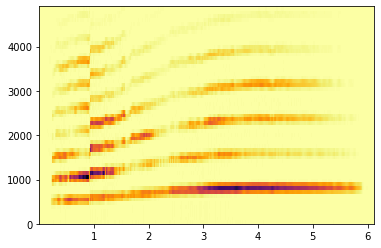
\includegraphics[scale=1]{fig/lab03/lab03_6.png}
		\caption{Спектрограмма сигнала}
	\end{center}
\end{figure}

Видим, что спектограмма очень похожа на наш чирп.

\subsection{Упражнение 5}

Тромбонист может играть глиссандо, выдвигая слайд тромбона и непрерывно дуя. По мере выдвижения ползуна общая длина трубки увеличивается, а результирующий шаг обратно пропорционален длине.
Предполагая, что игрок перемещает слайд с постоянной скоростью, как меняется ли частота со временем?

\noindent Напишите класс TromboneGliss, расширяющий класс Chirp и предоставляет evaluate. Создайте волну, имитирующую тромбон глиссандо от F3 вниз до C3 и обратно до F3. C3 — 262 Гц; F3 есть 349 Гц.

\begin{lstlisting}[language=Python]
class TromboneGliss(Chirp): 
    def evaluate(self, ts):
        lengths = np.linspace(1.0 / self.start, 1.0 / self.end, len(ts))
        freqs = 1 / lengths
        dts = np.diff(ts, prepend=0)
        dphis = np.pi * 2 * freqs * dts
        phases = np.cumsum(dphis)
        ys = self.amp * np.cos(phases)
        return ys
\end{lstlisting}

Создадим два сигнала-глиссандо от С3 до F3 и от F3 к C3 и соеденим эти два сигнала.

\begin{lstlisting}[language=Python]
firstSignal = TromboneGliss(262, 349)
firstWave = firstSignal.make_wave(duration=1)
spectr = firstWave.make_spectrogram(1024)
spectr.plot(high=1000)
\end{lstlisting}
\begin{figure}[H]
	\begin{center}
		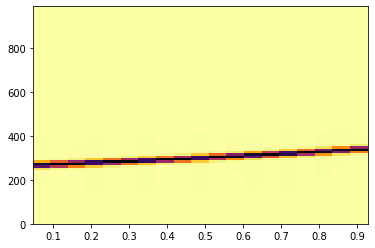
\includegraphics[scale=1]{fig/lab03/lab03_7.png}
		\caption{Спектрограмма первого сигнала}
	\end{center}
\end{figure}

\begin{lstlisting}[language=Python]
secondSignal = TromboneGliss(349, 262)
secondWave = secondSignal.make_wave(duration=1)
secondWave.make_audio()
spectr = secondWave.make_spectrogram(1024)
spectr.plot(high=1000)
\end{lstlisting}

\begin{figure}[H]
	\begin{center}
		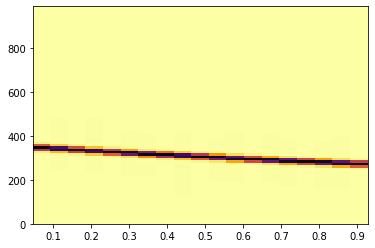
\includegraphics[scale=1]{fig/lab03/lab03_8.png}
		\caption{Спектрограмма второго сигнала}
	\end{center}
\end{figure}

Объеденим сигналы

\begin{lstlisting}[language=Python]
result = firstWave | secondWave
result.make_audio()
spectr = result.make_spectrogram(1024)
spectr.plot(high=1000)
\end{lstlisting}

\begin{figure}[H]
	\begin{center}
		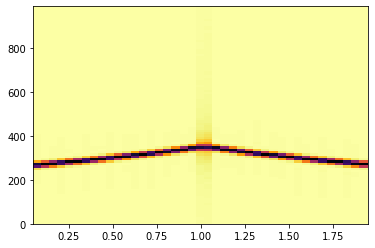
\includegraphics[scale=1]{fig/lab03/lab03_9.png}
		\caption{Спектрограмма объедененного сигнала}
	\end{center}
\end{figure}

Слышно, как две части идут друг за другом, также это хорошо видно на графике

\subsection{Упражнение 6}

Сделайте или найдите запись серии гласных звуков и посмотрите на спектрограмму. Сможете ли вы различить разные гласные?

Снова воспользуемся репозиторием учебника и возьмем оттуда звуки глассных.

\begin{lstlisting}[language=Python]
if not os.path.exists('87778__marcgascon7__vocals.wav'):
    !wget https://github.com/AllenDowney/ThinkDSP/raw/master/code/87778__marcgascon7__vocals.wav
wave = read_wave('87778__marcgascon7__vocals.wav')
wave.make_audio()
wave.make_spectrogram(1024).plot(1000)
\end{lstlisting}
\begin{figure}[H]
	\begin{center}
		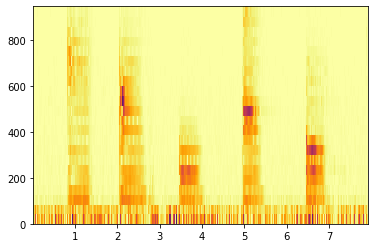
\includegraphics[scale=1]{fig/lab03/lab03_10.png}
		\caption{Спектрограмма гласных звуков}
	\end{center}
\end{figure}

На записи глассных есть 5 звуков и по спектограмме отчетливо видны эти глассные звуки в виде пиков.

\subsection{Вывод}

В данной работе были рассмотрены частотные компоненты и апериодические сигналы.
